% !TeX spellcheck = en_GB
\documentclass{acm_proc_article-sp} % alebo sig-alternate
\usepackage[english]{babel}
\usepackage[utf8]{inputenc}
\usepackage{url}
\usepackage{cite}
\usepackage{booktabs}
\usepackage{graphicx}
\usepackage{multirow}
\usepackage{tabulary}
\usepackage{tabularx}
\setlength{\heavyrulewidth}{1.2pt}
\setlength{\lightrulewidth}{0.7pt}



\begin{document}



\title{Detecting Search Sessions Using Document Metadata and
	Implicit Feedback}

\numberofauthors{2}

\author{
\alignauthor
Tomáš Kramár\\
       \affaddr{Institute of Informatics and Software Engineering
}\\
       \affaddr{Faculty of Informatics and Information Technologies
}\\
       \affaddr{Slovak University of Technology
}\\
       \affaddr{Bratislava, Slovakia
}\\
       \email{kramar@fiit.stuba.sk}
\alignauthor
Mária Bieliková\\
       \affaddr{Institute of Informatics and Software Engineering
}\\
       \affaddr{Faculty of Informatics and Information	Technologies
}\\
       \affaddr{Slovak University of Technology
}\\
       \affaddr{Bratislava, Slovakia
}\\
       \email{bielik@fiit.stuba.sk}
}

\maketitle

\begin{abstract}
	
It has been shown that search personalization can greatly
benefit from exploiting user’s short-term context – user’s
immediate need and intent. However, this requires that the
search engine must be able to divide user’s activity into segments,
where each segment captures user’s single goal and
focus. Several different approaches to search session segmentation
exist, each considering different features of the
queries, but it may be helpful to also consider user’s implicit
feedback on the search results clicked in response to
the query. We propose a method for segmenting queries into
search sessions which is based on document metadata and
incorporates implicit feedback. Our approach also considers
multitasking, where user shifts her current interest, but afterwards
proceeds with the original task. We evaluated our
approach on manually segmented query log and compared
the results of our approach with results from other methods
and showed that using implicit feedback can improve the
performance of the segmentation task.

\end{abstract}

\category{H.3.3}{Information Search and Retrieval}{Query formulation,
	Selection process, Search process
}

\terms{Information retrieval}

\keywords{personalization, search, short-term contexts, search sessions,
	search session segmentation}


\section{Introduction}

Web contains an ever-growing amount of documents. Accessing
these document poses great difficulties, especially
after the rise of Web 2.0 where users have been given the
ability to create the content, which allows for more socialbased
approaches to personalization \cite{Barla:1}, but also contributes
to information overload. According to Technorati1
, a service
which tracks user-generated media, the content on the Web
is growing with a pace at 2 blog posts per second, and this
number does not include the growth of other content.

Search engines play a crucial role in accessing this amount
of content. Users interact with search engines by entering
few keywords, which describe their intent and expect the
machine to provide a list of relevant documents. This model
has several known disadvantages:

\begin{itemize}  
	\item the number of keywords is usually low, typically 1-3
	keywords [17] and this often leads to ambiguity and
	unclear intent;
	\item many of the words are ambiguous; a word “jaguar”
	can refer to an animal, a car and even has less-known
	meanings such as a game console or German battle
	tank;
	\item the queries are almost never accurate \cite{Downey:2}, they are either
	too generic or too specific, but almost never exactly
	aligned with the specific intent the user has in
	mind.
\end{itemize}

The combined impact of these problems leads to a conclusion
that finding the relevant document when we do not have
enough information about it is indeed a difficult task, both
for the user and the search engine.

To mitigate this problem, several approaches to search personalization
have been researched, each with the ultimate
aim to help users find the relevant content, without trying
to change how humans think, or work.

There is relevance feedback, query expansion, search intent
detection, alternative ranking schemes and many others.
These techniques leverage and act upon some form of search
context. Generally, the term context refers to attributes of
the environment \cite{Dourish}, such as location, time, or weather, but
in the domain of personalized search the term is commonly
used to describe user’s needs, goals and intents (e.g. [21, 27]).
Based on the time span that is used to build the search context,
the context may be long, or short-term.

Long-term search context is composed of the goals and intents
that can be recognized by observing the complete user
activity, beginning with the first known information about
the user and her activity.

Short-term search context is composed of the goals and intents
that the user has in the moment of search. These
represent the current focus and are obtained by observing
the user activity beginning in a recent point of time.

To be able to use short-term search context a personalization
system must know the exact moment the user changes
her intent, so that it can start and use a new context. The
task of detecting this change is referred to as search session
detection (segmentation). The term search session was
never formally defined in the literature and its meaning differs
in different works. In this work, we assume that search
session is a sequence of search related actions with the single
underlying informational intent, similarly to [22].

The goal of search session segmentation is to partition the
stream of user queries into segments of queries, where each
segment is the search session, i.e., holds the condition that
all queries that it contains are related to a single underlying
goal.

Several existing approaches to search session segmentation
exist, but they have various disadvantages. When a segmentation
approach acts solely on the features provided by the
query itself, the amount of understanding of the underlying
intent is quite limited. Therefore, many approaches also
consider the documents that were clicked in response to the
query, but these approaches do not evaluate user’s feedback
that is implicitly left in each document. Many existing approaches
also do not consider interruptions in Web browsing
and multitasking (i.e. having multiple intents).

In this work we aim to contribute to the area of search session
segmentation by matching the queries with the metadata
of the documents clicked from the search results to get
better insight into the purpose of the query by aggregating
more data than only the query itself provides. We also
evaluate the level of page usefulness for the particular query
by collecting and analyzing the implicit feedback indicators
that the user provides for each page view. Our approach
also considers user interruptions and is able to separate intermingled
sessions and reconnect interrupted sessions.

The paper is structured as follows. Section 2 describes the
related work done in the area of search session segmentation.
In Section 3 we describe our data collection methodology.
Section 4 describes the proposed method for search
sessions segmentation. Experimental results are described
in Section 6.

\section{RELATED WORK}

The most widely used approach to search session segmentation
is to compare temporal distance of the queries. If two
queries were issued with a time difference larger than a predefined
threshold, it is assumed that a new session started,
and the existing session is split at that place. This technique
was first described in \cite{Catledge:1}, establishing the threshold
of 25.5 minutes. They measured an average time between
page requests (9.5 minutes) and added a 1.5 standard deviation.
This approach only makes sense for normal distribution,
while surfing on the Web shows properties of a long-tail
distribution. The established 25.5 minutes are part of the
long-tail distribution and it wouldn’t make much difference
if 20, or 40 minutes were used instead [14]. He et al. [13] experimented
with various cutoff settings and established that
the optimal cutoff time is between 10 and 15 minutes. Due
to its simplicity both in concept and implementation, this
technique is widely used and there are modification ranging
from use of 5 minutes cutoff \cite{Downey:1}, through 30 minutes cutoff
[24] to a per-user cutoff [23].

\begin{itemize}  
	\item it is unable to detect sessions which are split within
	a short time – if the search intent changes quickly,
	without sufficient time passing between consecutive
	queries, the queries are falsely considered as part of
	a single session, yet they might bear a different underlying
	intent;
	\item the long time between searches may not mean that the
	user’s intent changed – this is a well known downside
	of any time-window based method. The longer pause
	between queries may be caused by several factors, such
	as reading long article, breaks, or any other interruptions
	that are commonly encountered nowadays \cite{Coplien:MPD}.
\end{itemize}

Another approach uses lexical distance of the queries. This
idea compares content of two queries to detect if the intent
has changed. Example of this approach is stated in [16].
The main drawback of this method is that it leads to a high
amount of false positives. There are many instances where
two queries are completely dissimilar (they share no common
words), yet their underlying intent is the same. Consider
a user searching for “IR” and “information retrieval”
afterwards. Using the lexical distance approach would incorrectly
yield two separate sessions.

Method described in [11] combines both temporal and lexical
distances. They use vector-space representation, where each
pair of following queries is placed in the space. If the query
pair fits into the space bounded by the subplane delimited
by two edge cases

\begin{itemize} 
	\item two parallel, but dissimilar queries,
	\item the same queries, but executed long time apart
\end{itemize}

it is considered an extension of the current session. Although
this combination can achieve better results than each of the
methods alone, it is still prone to the aforementioned problems.

As stated, related queries do not provide sufficient data to
match similar intents, but there are approaches that use
signals from the retrieved documents. In [25], authors used
vectors of titles and snippets of 50 top-ranked documents
for the query. The session is split as determined by comparing
cosine similarities of two following queries. Another
approach uses document keywords. In \cite{Daoud:1}, authors extract
document’s keywords using the TF.IDF scheme and map
them to ODP categories. The session is then split when the
ODP category changes. This approach however fails to account
for user’s real interests. When the user enters a query
and clicks and views some documents only to realize that the
results are wrong and the query needs to be reformulated,
this approach has already used these faulty results to decide
upon session segmentation.

Jones and Klinker [18] trained a binary classifier to detect
whether two queries are part of the same search task or not,
using a set of syntactic, temporal, query log and web search
features. They have obtained best results by incorporating
a vector derived from the first 50 results for the given query,
but this approach again suffers from the query ambiguity.

Currently, the arguably best approach is grouping related
queries into sessions by using a clustering methods. The
key feature of the approach is wikification of the queries,
i.e., building a relevance vector in a high dimensional concept
space of Wikipedia articles [22]. The relevance vector
describes relevance of the query terms for each Wikipedia
article. Although this approach gives good result on the
manually annotated set of circa 1300 queries, it is strongly
dependent on the Wikipedia articles. Given a query which
does not contain a term present on Wikipedia, this approach
does not yield any benefit over other methods. Our method
is not dependent on other external and limited knowledge
base, instead, it depends only on clicked search results which
follow naturally after every search.

Most of the existing approaches also do not deal with multitasking.
Multitasking might be present in several forms,
mainly:

\begin{itemize} 
	\item parallel browsing, when a user is having multiple goals
	at the same time and working on them at the same
	time by means of having multiple browsers, or multiple
	browser tabs, or
	\item browsing with interruptions, when a user is having a
	single goal but is interrupted, switches the goal for a
	while and returns back to the original goal afterwards.
	The interruption may not be forced, it may be the
	user’s conscious decision to abandon the current task
	and concentrate on different goal.
\end{itemize}

The practical effect of multitasking on search session segmentation
is that it is causing the sessions to be disconnected.
Single search session is interrupted by queries that
are part of another session and then the session continues,
as the user returns to the original goal.

There are mixed reports on the presence of multitasking on
the Web. According to [15] only 25% of users multitask.
When searching, the multitasking is practically nonexistent
for navigational and transactional queries [28], it is only
present in 6-15\% of ambiguous queries. Older study \cite{Buzikashvili:1} reports
that only 1\% of all sessions are diconnected. Lucchese
et al. analyzed AOL query log and report that multitasking
in search exists [22].

In \cite{Buzikashvili:1} a method to detect disconnected sessions is proposed.
Their approach is executed in two steps: in the first phase,
sessions are segmented using a cutoff time, in the second
step, all queries in each session are compared to build a similarity
graph where the transitive closure is computed. All
queries connected by the closure are considered part of the
same session. This approach again combines the disadvantages
of the approaches it merges – temporal and lexical
distance. In [22] the queries are connected using clustering
methods, so the multitasked queries are connected naturally.

Our work extends and differs from existing research in several
important ways


\begin{itemize} 
	\item First, we only consider the documents that the user
	deemed useful. To measure the usefulness, we partially
	rely only on the clickthrough data and only consider
	the search results that the user actually viewed, but
	we also use implicit feedback indicators to weight the
	contribution of each of the documents.
	\item The search sessions are segmented by comparing their
	metadata (both machine and human extracted), and
	to increase the chance of a successful match, we extend
	the metadata with ConceptNet relations.
	\item Our approach also considers multitasking and user interruptions
	– we maintain a stack of short contexts
	(search sessions) and when the query fits within a previously
	abandoned session, this session can be popped
	from the stack and continued.
\end{itemize}

\section{DATA COLLECTION}

Our work is based on the idea of considering only the documents
that the user found useful, therefore we need a way
to collect user’s actions on search engine and implicit feedback
on viewed documents \cite{XFu:1}. In order to gain detailed
insight into users actions and to collect precise and rich implicit
feedback data, we leverage a personalized proxy server,
called PeWe Proxy. The collection process is described in
more detail in Fig. 1.

The personalized proxy server2
acts as a regular proxy, sitting
between the user and the Web [20]. All user’s requests
are handled by the proxy first and then forwarded to the
target server. Similarly, the response from Web server has
to pass through the proxy. This means that the proxy has
access to complete message processing between client and
the server and can even modify the actual content of the
request/response.

We are aware, that using proxy server in a production search
engine is not a realistic option. We are using proxy server to
gain detailed insight into implicit feedback on every accessed
page. Some level of implicit feedback can be inferred by
analyzing timestamps and patterns in query logs [26].

\begin{center}
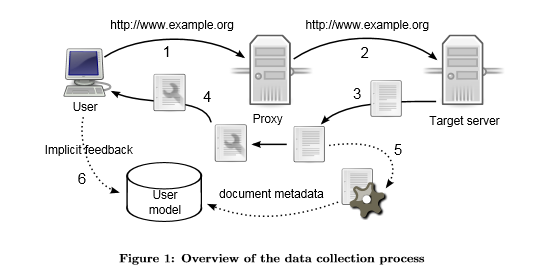
\includegraphics[width=90mm]{DataCol.png}

\end{center}



\subsection{Implicit feedback collection}

We use the proxy server to inject a tracking JavaScript into
each page, which collects the following implicit feedback signals:

\begin{itemize} 
	\item \textit{real time spent on page} – the actual time spent on page
	is measured in series of short time windows. If there
	is an observed activity within the page (i.e., mouse
	movement, scrolling, clicking, writing) during the span
	of the window, the length of the window is added to the
	total time on page. In this case, we used the window
	of 4 seconds;
	\item number of clicks, scrolls and copying into clipboard;
\end{itemize}

\subsection{Metadata collection}

Besides the implicit feedback collection, we use PeWeProxy
to create logs of user activity, i.e., we track the documents
that the user visited and to associate each log with its corresponding
implicit feedback signals.

Each document is processed and following types of metadata
are extracted:

\begin{itemize} 
	\item \textit{keywords} – we extract keywords automatically by using
	the tagthe.net and Alchemy Orchestr8 Web services
	and JATR library;
	\item \textit{tags} – we use human created directory of tags, the Web
		service delicious.com;
	\item \textit{named entities} extracted by using \textit{OpenCalais} Web
		service;
	\item \textit{categories} from the human-maintained project ODP
\end{itemize}

All metadata is extracted by using a wrapper Web service
Metall3
, which strips the document from auxiliary content
(ads, menus, header, footer, etc.), leaving only the main text
of the document, which is translated into English and the
described services are used to extract metadata. We translate
the documents into English, as the available extraction
services work best with English text. The automatic translation
is far from perfect, but the basic informational structure
of the text is retained and as our previous experiments show,
the quality of metadata extracted from translated texts is
satisfactory \cite{Barla:2}.

\section{SEGMENTING SEARCH SESSIONS}

Our method of search session segmentation operates in the
following steps:

\begin{enumerate} 
	\item building candidate search results for the intent model
	of the query
	\item pruning the candidates by the implicit feedback indicators
	\item using the intent models to match the queries to discover
	sessions
\end{enumerate}

\subsection{Building the intent model of the query}

For each query, we find the candidate set of useful documents.
These are the documents that were clicked from the
search engine results page. We use the value of referrer
HTTP header – each Web page that was followed from the
search engine results page would have the results page URL
address as referrer.

The basic assumption behind this filtering is that users only
click at the results that help them fullfil their search goal (intent)
and extracting features only from these documents, as
opposed to extracting features from all documents retrieved
for the query will result in having a more accurate intent
model.

However, the pruned set of documents only represents the
candidates, as they

\subsection{Pruning by implicit feedback indicators}

To further prune the documents that were viewed in response
to the search query, we consider the implicit feedback
indicators. This helps us to remove search hits that

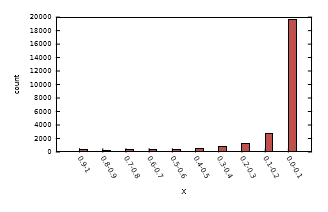
\includegraphics{Graph1.png}
\textbf{Figure 2: Distribution of the implicit feedback values over the search result hits accessed via the proxy server.}

were clicked, but did not really contribute to the fullfilment
of the underlying intent. A typical example is an ambiguous
query (e.g. jaguar), which yields documents that cover
wide range of topics. The user, biased by the search engine
ranking [19], may click the search result dealing with wrong
topic. Similarly, a user willing to buy a car might formulate
a vague query including model of a car and hit a wide variety
of search results dealing with reviews, descriptions or
car shops offerings.

Again, we make the basic assumption that upon visiting a
page which does not conform to the underlying search intent,
the user expresses lower level of interest. We estimate the
level of interest via the level of interaction which is captured
in form of the various implicit feedback indicators. The particular
indicators are aggregated and final value of implicit
feedback (X ) is calculated as

\begin{equation}w = \frac{time on page + click cnt + copy cnt + select cnt}{content length}\end{equation}

which is then normalized as

\begin{equation}X = 1 - \frac{1}{1 + w}\end{equation}

We arbitrarily weight the indicators equally. Figure 2 shows
the distribution of X calculated for all search results accessed
via the proxy over the period of one year. This distribution
exhibits the long tail property, with the majority
of Web pages with the value of 0 < X > 0.1.

We prune all accesses with the value of X < Xmin.

\subsection{ Matching the sessions}

Each query q is associated with a set of relevant documents
Q = {Dq,1, Dq,2, . . . , Dq,n} that were clicked in response to
the query and passed the implicit feedback filters. Each
search result (document) for query q is modeled as a set of
metadata Dq,i = {m1, m2, . . . , mm}.
The intent model of the query q is calculated by unioning
all document models as follows:

If there is a query which has no document views associated
with it (either there was no click on the search engine results
page, or all clicks were pruned by the implicit feedback level
restriction window) then its intent model is represented as
an empty set.
After the final step, each query has associated a set of metadata
which describes the search results that the user found
interesting. We also build a second set of enhanced metadata
for each query by querying the ConceptNet [12] API
for related terms for each term in the original intent model.

The log segmentation then proceeds as follows:


\begin{enumerate} 
	\item The queries are ordered by the date they were issued
	\item The session stack T, which is used to store recent sessions
	is initialized to empty stack
	\item  Starting with oldest query, the log is processed
	\item  The stack T is traversed top-down, starting with the
	most recent session and each session Sc is examined
	\item  The intent model of the query q is compared with the
	session model Sc. If there is a significant match between
	the metadata terms in session model and query
	intent model, i.e.
	\begin{equation} I_{q} = \bigcup_{i=1}^{n} D_{q,i} \end{equation}
	then the query q is considered part of the session Sc.
	The intent model of the query is merged into the session
	model:
	\begin{equation} \left \| S_{c} \cap I_{q} \right \| > sim_{min} \end{equation}
	The session Sc is removed
	from the stack and added at the top, as the most recent
	session. The processing continues with next query
	at step 3.
	\item When all sessions from the stack were examined and
	none was matched by the current query q, the query is
	considered the beginning of a new session. New session
	Sc is created as Sc = Iq and added on top of the session
	stack T. Processing of the log continues at step 3.
\end{enumerate}

Maintaining the session stack T is the key part, that allows
the method to consider multitasking and interruptions.
When the user changes context but then returns back to the
original context, we are able to link the following actions to
the original context. For practical reasons and to prevent
the queries to rejoin old sessions, the stack only accepts sessions
that are not older than Told. The age of the session
is calculated as the time when the oldest query from that
session was issued.

\section{EVALUATION}

To evaluate our approach to search session segmentations,
we used a log of searches collected on the proxy platform
over the period of 4 days. We analyzed all search requests to
Google search engine, and automatically filtered all queries
that were automatically issued by the browser to autocomplete
the search, when the user is typing the query or location
into the address bar. The final filtered query log contains
245 queries from 3 different users. To obtain a baseline
to compare against, these queries were manually segmented
into search sessions by a human evaluator. To remove a
possible time bias, the segmentation user interface did not
contain information about the time of query – only the text
of the query itself.

The main problem of evaluating session segmentation is that
it is often hard, even for human evaluators, to detect the
similarities and intents behind the queries. When searching,
users describe the problem domain with short keywords, so
often a thorough knowledge of the problem domain is required,
to decide what is similar and what not. Table 1
shows some examples from the analyzed query log. This implicates
that even the manually segmented sessions may be
incorrect.

For the experiment setup, we initialized the parameters as
shown in Table 2.

\begin{table}[]
	\centering
	\caption{Initial parameters used in the experiment}
	\label{my-label}
	\resizebox{0.4\textwidth}{!}{%
		\begin{tabular}{|p{4.5cm}|p{4.5cm}|p{4.5cm}|}
			\hline
			\begin{math}
			T_{old} = 1 day 
			\end{math}    
			                            & disconnected session older than 1 day will not be rejoine                                                                                                                                                              \\ \hline
			\begin{math}
			X_{min} = 0.1
			\end{math}
			 				            &all documents with implicit feedback value lower than 0.1 are considered irrelevant, 
			                            this value was selected according to the long-tail distribution of implicit feedback over the searchresults                    
			                            \\ \hline
			\begin{math}
			sim_{min} = 4 
			\end{math}
			                            & the intent models of two queries must match at at least 4 terms                                                                                                                                                        \\ \hline
		\end{tabular}%
	}
\end{table}

Table 3 summarizes the results obtained with various segmentation
methods. Approach in the table refers to the specific
method that was used to segment the logs. In lexical
approach, we used query similarities – two following queries
sharing at least one common keyword were considered to be
part of the same session. Temporal approach refers to time
based similarity. The number in the name indicates the size
of the cutoff window used. Temporal30m means that queries
were segmented by using a 30 minutes inactivity cutoff time,
temporal5m uses a 5 minute cutoff. In metadata we compared
similarity between the sets of query metadata – for
two following queries, if the intersection of their metadata
sets was non-empty, the queries were considered part of the
same session. Similarly enhanced metadata compares sets of
ConceptNet enhanced metadata.

To evaluate the quality of each approach, sessions were compared
to the baseline (manually created sessions) and precision
and recall were calculated using the following methodology:

Precision indicates the internal coherence of the session.
Queries from automatically detected session are mapped to

the manually detected sessions and precision is calculated as
the ratio of the cardinality of the best match (i.e. the most
frequent session in the mapping) to the cardinality of the
whole session.

For example, the query log contains queries

{A, B, C, D, E, F, G, H, I}

The human evaluator segmented the log into two sessions:

H1 : {A, B, C, G, H, I}
H2 : {D, E, F}.

The automatic method detected three sessions:

A1 : {A, B, C, D}
A2 : {E, F}
A3 : {G, H, I}

Queries from automatically detected sessions are mapped to
their manually created sessions, yielding:

A1 : {H1, H1, H1, H2}
A2 : {H2, H2}
A3 : {H1, H1, H1}

For A1, the best match is H1, as is contains three queries
from H1 as opposed to one query from H2. The cardinality
of the best match is 3, cardinality of the whole session is 4,
the precision is thus 3/4.

Recall indicates the completeness of the session. It is calculated
as the ratio of cardinality of the best match against
the manually created sessions to the cardinality of the bestmatched
session. In the above example for A1, the session
H1 (best match for A1) contains 6 queries, cardinality of the
best match is 3, the recall is thus 3/6.

We see that when using the classical methods, the lexical
approach outperforms temporal methods, with the widely
used 30 minute cutoff yielding slightly better performance.
Metadata based approach did not outperform temporal approaches
and yielded low recall. This is due to the fact that
the extracted metadata generally cover wide area of topics
and metadata from similar pages on the same topic do not
necessarily overlap.

We expected that enhancing the metadata would improve
performance by connecting similar words and improving the
chance for a match, yet the performance of the enhanced
metadata was worse than that of the metadata alone. This
is rather surprising, but after closer inspection of the metadata
and ConceptNet connections, we believe that this was
caused by several factors:

\begin{itemize} 
	\item queries were generated by technical users who deal
	with specific technologies and problems which include
	vocabulary not present in the ConceptNet database –
	the majority of metadata was thus left unexpanded;
	\item in many cases, the ConceptNet relations are too general
	and at very different conceptual levels (e.g. the
	term “jaguar” is linked to term “black”) – in turn, the
	query metadata was enhanced with many generic and
	abstract terms, leading to a false positive matches thus
	reducing precision and recall.
\end{itemize}


\begin{table}[ht!]
	\centering
	\caption{Examples of difficult search sessions from a real query log}
	\label{my-label2}
	\resizebox{0.5\textwidth}{!}{%
	\begin{tabular}{|ll|}
		\hline
		\multicolumn{1}{|l|}{queries, separated with semicolon} & reason of similarity                \\ \hline
		magneto-dynamic pickup; psg4003                         & psg4003 is a magneto-dynamic pickup \\
		makarska; saint tropez, costa del sol                   & all three are summer resorts        \\
		usb phonograph; l3866usb                                & l3866usb is an usb phonograph       \\
		the ills; youcoco                                       & both are music bands                \\ \hline
	\end{tabular}%
    }
\end{table}


Next, we focused on evaluating the interruptions. The combined
approach of using lexical similarity with interruption
detection slightly outperformed lexical similarity alone. We
tried to limit the stack traversal to sessions created in last
0.5, 2 and 8 hours by modifying parameter Told, but this
approach did not yield an improvement.

On closer inspection of the results, we noticed that the metadata
based approach excels at linking queries where lexical
similarity fails (see Table 1 for examples). We combined the
two approaches, and employed the metadata based similarity
only when the lexical similarity did not find a match.
This approach yielded the best score.

\section{CONCLUSIONS AND FUTURE WORK}

to the query – we discard badly formulated queries or misleading
search results. Our approach is also able to detect
and link interrupted sessions, by maintaining and searching
a stack of past sessions.

We present the results of an evaluation on the set of manually
segmented queries. We’ve shown that considering interruptions
can improve the performance of lexical similarity
and that we can achieve best results when combining lexical
similarity with metadata similarity, as this approach can
correctly link queries, which are hard to link even for human
evaluators, not even the lexical approach. This study
has warranted the validity of our approach and confirmed
that using implicit feedback, metadata and interruptions is
a promising research area.

In the next work, we will focus on building a larger dataset
of manually segmented sessions. We plan to use the personalized
proxy server platform to allow users themselfs to
segment their own sessions as they search. We also plan on
evaluating other means of enhancing the document metadata,
e.g. by using automatically generated hypernyms.

\textit Acknowledgement

This work was partially supported by the grants VG1/0675/
11/2011-2014, APVV-0208-10 and it is the partial result of
the Research and Development Operational Programme for
the project Research of methods for acquisition, analysis
and personalized conveying of information and knowledge,
ITMS 26240220039, co-funded by the ERDF.


\bibliographystyle{abbrv}
\bibliography{literatura}



\balancecolumns

\end{document}
